% ============================================================
%  Artículo Técnico — Formato IEEE Conference
%  Sistema Inteligente para la Identificación y Seguimiento
%  de Derechos de los NNA por Feminicidios
%  Escuela Superior de Cómputo — I.P.N.
% ============================================================
\documentclass[conference]{IEEEtran}

% ── Paquetes ─────────────────────────────────────────────────
\usepackage[spanish,es-tabla]{babel}
\usepackage[utf8]{inputenc}
\usepackage[T1]{fontenc}
\usepackage{graphicx}
\usepackage{amsmath}
\usepackage{amssymb}   % define \checkmark
\usepackage{booktabs}
\usepackage{array}
\usepackage{url}
\usepackage{cite}
\usepackage[hidelinks]{hyperref}
\usepackage{listings}
\usepackage{xcolor}

% ── Estilo para bloques JSON ─────────────────────────────────
\lstdefinelanguage{json}{
  basicstyle=\ttfamily\scriptsize,
  showstringspaces=false,
  breaklines=true,
  frame=single,
  rulecolor=\color{black!40},
  backgroundcolor=\color{gray!6},
  stringstyle=\color{black},
  morestring=[b]",
  literate=
   *{0}{{\color{blue!70}0}}{1}
    {1}{{\color{blue!70}1}}{1}
    {2}{{\color{blue!70}2}}{1}
    {3}{{\color{blue!70}3}}{1}
    {4}{{\color{blue!70}4}}{1}
    {5}{{\color{blue!70}5}}{1}
    {6}{{\color{blue!70}6}}{1}
    {7}{{\color{blue!70}7}}{1}
    {8}{{\color{blue!70}8}}{1}
    {9}{{\color{blue!70}9}}{1},
}

% ── Forzar "Resumen" y "Palabras clave" en lugar de Abstract / Index Terms ──
\renewcommand{\abstractname}{\normalfont\textbf{Resumen}}
\newcommand{\keywordsname}{\normalfont\textbf{Palabras clave}}

% ── Subsecciones con letra mayúscula (A. B. C. ...) ──────────
% IEEEtran usa \alph por defecto en modo conference; se fuerza aquí.
\renewcommand{\thesubsection}{\Alph{subsection}}

% ── Tablas en mayúsculas estilo IEEE ("TABLA I") ─────────────
\addto\captionsspanish{\renewcommand{\tablename}{TABLA}}
\renewcommand{\thetable}{\Roman{table}}

% ── Figuras ──────────────────────────────────────────────────
\addto\captionsspanish{\renewcommand{\figurename}{Fig.}}
\renewcommand{\thefigure}{\arabic{figure}}

% ── Macros de conveniencia ───────────────────────────────────
\newcommand{\BETO}{\textsc{beto}}
\newcommand{\NNA}{NNA}

% ============================================================
\begin{document}

% Usando \large (Tamaño mediano) y negritas
\title{\large\bfseries Sistema Inteligente para la Identificación y Seguimiento
       de Derechos\\de los NNA en Situación de Orfandad por Feminicidio}


% ── Autores — bloque centrado en 3 líneas ────────────────────
\author{%
  Héctor Alberto Morales Martínez,\ M. en C. Ulises Saldaña Velez,\ M. en C. Gabriel Hurtado Avilés\\
  Escuela Superior de Cómputo\ I.P.N.\ México CDMX\\
  \textit{Tel. 5616148167. E-mail: \href{mailto:hmoralesm1500@alumno.ipn.mx}{hmoralesm1500@alumno.ipn.mx}}%
}
 
\maketitle

% ── Resumen ────────────────────────────────────────────────── 
\begin{abstract}
Se presenta el diseño, desarrollo y evaluación de un sistema inteligente
orientado a identificar y dar seguimiento de las Niñas, Niños y Adolescentes
(\NNA{}) en situación de orfandad derivada de feminicidios en México. El
sistema integra una arquitectura de microservicios contenerizada en Docker
compuesta por tres módulos principales: (1)~un recolector multi-fuente basado
en \texttt{StealthSession} con emulación de firma TLS/JA3 para evadir
contramedidas perimetrales en 45~fuentes RSS y Google News;
(2)~un clasificador neuro-simbólico escalonado de cuatro capas que combina
el modelo Transformer \BETO{} con ajuste fino supervisado
(\textit{fine-tuning}) y reglas heurísticas con penalizaciones y
bonificaciones aditivas para neutralizar el denominado
\textit{efecto péndulo}; y (3)~un módulo de agrupamiento semántico basado
en BERTopic (UMAP~+~HDBSCAN~+~c-TF-IDF) y un investigador profundo
(\textit{DeepInvestigator}) accionable bajo demanda que sintetiza fichas
de caso estructuradas mediante la API de Gemini~Flash.
La cascada de deduplicación de cuatro fases (MD5, Jaccard, SimHash y coseno
TF-IDF) depuró 213~duplicados, resultando en 634~noticias únicas procesadas.
Sobre un conjunto de prueba ciego de 41~noticias etiquetadas con acuerdo
inter-anotador $\kappa{=}0.91$, el clasificador alcanzó F1-Score~=~0.85,
Recall~=~0.95 y tasa de falsos positivos del 30\%, cumpliendo el umbral
operativo establecido. Los resultados demuestran que la integración de
razonamiento simbólico sobre el componente neuronal es esencial para dominios
de alta especificidad semántica como la violencia de género y la protección
de la infancia.
\end{abstract}

% ── Palabras clave ───────────────────────────────────────────
\vspace{4pt}
\noindent\keywordsname\ ---
Procesamiento de Lenguaje Natural, Web Scraping, BERT, BERTopic,
Clasificación Neuro-Simbólica, Feminicidio.

% ============================================================
\section{Introducción}

México atraviesa una crisis documentada de violencia feminicida, el
Secretariado Ejecutivo del Sistema Nacional de Seguridad Pública (SESNSP)
registra más de 8\,000 víctimas de feminicidio entre 2010 y
2023~\cite{sesnsp2023}. La Red por los Derechos de la Infancia en México
(REDIM) estima que al menos 3\,500 \NNA{} perdieron a su madre como
consecuencia directa de estos crímenes~\cite{redim2022}. A pesar de la
gravedad de esta cifra no existe a nivel nacional un padrón oficial ni un
mecanismo estandarizado que documente el estado de estas víctimas indirectas.

La Convención sobre los Derechos del Niño y la Ley General de los Derechos
de Niñas, Niños y Adolescentes (LGDNNA) establecen el principio del
\textit{interés superior de la niñez} como eje principal, sin embargo, la
ausencia de datos estructurados imposibilita su materialización
efectiva~\cite{onu2019}.

\subsection{Limitaciones del monitoreo manual}

La atención de esta invisibilidad estadística recae actualmente sobre
organizaciones de la sociedad civil. La metodología actual presenta un
cuello de botella operativo puesto que requiere la revisión manual de
fuentes hemerográficas. Con más de 1\,200 medios periodísticos digitales
activos en el país, el factor humano introduce una latencia que provoca
que numerosos casos pasen desapercibidos. Como consecuencia, el talento
humano especializado es desviado hacia tareas de recolección de datos
en lugar de la intervención directa con las víctimas.

\subsection{Contribución del trabajo}

El Trabajo Terminal 2026-A135 propone una solución tecnológica que automatiza
el ciclo completo de descubrimiento informativo. A diferencia de trabajos
previos basados en expresiones regulares~\cite{bird2009nlp} o vectorización
TF-IDF estática~\cite{joachims1998text}, la arquitectura propuesta combina
un modelo Transformer bidireccional con reglas simbólicas de dominio para
resolver la ambigüedad semántica inherente al periodismo policial mexicano.

% ============================================================
\section{Metodología}

El sistema fue desarrollado bajo un enfoque \textbf{evolutivo basado en
prototipos}~\cite{pressman2014}, dado la alta incertidumbre tecnológica en
dos frentes como lo son las infraestructuras dinámicas de evasión web
(WAF, JA3 fingerprinting) y la alta variabilidad e inferencia de los
modelos Transformer. Cuatro prototipos sirvieron como entornos de diagnóstico;
la iteración final constituyó el estado de producción.

\subsection{Recolección multi-fuente}

Los prototipos iniciales utilizaron \textit{BeautifulSoup} sobre
peticiones HTTP directas, obteniendo bloqueos HTTP~403 en el 80\% de las
fuentes por \textit{TLS/JA3 fingerprinting}~\cite{anderson2019tls}.
El módulo \textit{StealthSession} resolvía esto mediante
la emulación de fingerprint TLS vía \textit{cloudscraper} con hashes JA3
idénticos a Chrome/Windows; con delays log-normales ($\mu{=}2.5$,
$\sigma{=}0.7$, mediana $\approx$12.2\,s) que imitan comportamiento humano;
y un \textit{Circuit Breaker} por dominio que detiene las peticiones tras
tres fallos consecutivos.

El recolector scrapea 45~feeds RSS nacionales, Google News y fuentes
complementarias mediante scraping HTML, procesando $\approx$900~noticias brutas
por ciclo. La cascada de deduplicación de cuatro fases
(MD5~$\rightarrow$ Jaccard~$\rightarrow$ SimHash~$\rightarrow$ coseno TF-IDF) elimina un aproximado del 25\% del
corpus, entregando al módulo clasificador noticias únicas.

\subsection{Clasificador neuro-simbólico escalonado}

El motor de clasificación opera en cuatro capas autónomas y secuenciales.
La Fig.~\ref{fig:clasificador} ilustra el flujo completo.

\textbf{Capa~0. Escudo léxico.} Filtro de rechazo temprano $O(1)$
mediante \textit{frozenset} de dominios ajenos (deportes, economía,
tecnología). Única capa con bloqueo absoluto (\texttt{score~=~0}).

\textbf{Capa~1. Escudo suave.} Términos legislativos y
estadísticos aplican penalización aditiva $\delta{=}{-}0.35$ sin
bloquear la noticia. Una noticia con score BETO de 0.72 que menciona
``según datos del REDIM'' obtiene score ajustado de 0.37
(\textit{Media}). 

\textbf{Capa~2. Inferencia BETO.}
(\textit{bert-base-spanish-wwm-cased}) es un Transformer bidireccional
con 110 millones de parámetros, 12 capas de autoatención y embeddings de
768 dimensiones, preentrenado sobre Wikipedia en español mediante
MLM~\cite{CaneteCFP2020}. El \textit{hidden state} del token
\texttt{[CLS]} se extrae como representación global normalizada con
norma~L2. El sistema opera en modo \textit{Finetuned} (prioritario).

\textbf{Capa~3. Post-filtro heurístico.} Aplica bonificaciones
(+0.10 a +0.25) al detectar patrones de orfandad real
(\texttt{quedó al cuidado}, \texttt{menores bajo resguardo},
\texttt{hijos quedaron}) y penalizaciones para roles invertidos
(menor como agresor). Esta capa nunca produce exclusiones absolutas
para noticias \textit{Media}.

El score final acumulado que determina la clasificación de una noticia
se expresa formalmente como:
\begin{equation}
  S_{\text{final}}(x) = P_{\text{BETO}}(x) + \sum_{i} \delta_{i}(x)
  \label{eq:score}
\end{equation}
donde $P_{\text{BETO}}(x) \in [0,1]$ es la probabilidad de relevancia
emitida por el modelo Transformer y $\delta_{i}(x) \in \mathbb{R}$ son
las penalizaciones o bonificaciones aditivas aplicadas por las capas
simbólicas 0, 1 y~3 en función del contenido textual de $x$.

\begin{figure}[htbp]
  \centering
  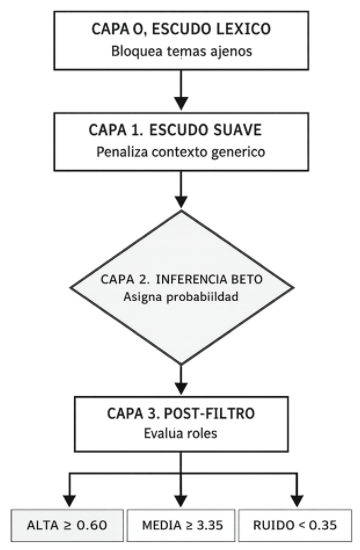
\includegraphics[width=\linewidth]{estructura.png}
  \caption{Arquitectura del clasificador neuro-simbólico escalonado de
           cuatro capas. Las capas simbólicas (0 y 1) modulan la
           salida neuronal de \BETO{} (Capa~2) mediante penalizaciones
           y bonificaciones aditivas antes del post-filtro (Capa~3).}
  \label{fig:clasificador}
\end{figure}

Este diseño neuro-simbólico neutraliza el \textbf{efecto péndulo}
observado en el prototipo 3, donde \BETO{} clasificaba erróneamente
discursos normativos con scores de hasta 0.81 por correlación
superficial de tokens.

\subsection{Agrupamiento Semántico BERTopic}

El flujo de BERTopic (UMAP~+~HDBSCAN~+~c-TF-IDF) procesa las
noticias únicas sobre embeddings \BETO{} de 768~dimensiones
reducidos a 5D por UMAP~\cite{bertopic2022}. Se generaron tópicos
semánticos coherentes (casos con intervención del DIF, disputas por
custodia, \NNA{} testigos, manifestaciones de colectivos). El Silhouette
Score mejoró de 0.23 (K-Means TF-IDF, P2) a una coherencia
cualitativa verificable sobre el espacio semántico de 768~dimensiones.

\subsection{Módulo DeepInvestigator} 

El módulo \texttt{DeepInvestigator} se activa bajo demanda desde el
dashboard sobre noticias de clasificación \textit{Alta}. Ejecuta cuatro
pasos que son la generación de un query de alta especificidad vía Gemini~Flash;
búsqueda dual en DuckDuckGo HTML y Lite; scraping complementario
con \textit{StealthSession}; y síntesis estructurada en JSON con
siete campos (\textit{ubicacion}, \textit{victimas},
\textit{ninos\_afectados}, \textit{edades}, \textit{situacion\_actual},
\textit{medios\_contacto}, \textit{resumen}). El campo
\textit{medios\_contacto} retorna como recomendacion de contacto a institucione
como el DIF municipal y la Fiscalía
competente según la ubicación del caso. Tiempo promedio:
\textbf{47~segundos por caso}.

El siguiente ejemplo ilustra una ficha de caso representativa generada
por Gemini~Flash (datos completamente anonimizados):

\begin{lstlisting}[language=json,caption={Ejemplo de ficha JSON generada por DeepInvestigator (anonimizado).},label={lst:json}]
{
  "ubicacion": "Municipio de [ANONIMIZADO], Estado de [ANONIMIZADO]",
  "victimas": "Mujer adulta, 32 años",
  "ninos_afectados": 2,
  "edades": ["7 años", "11 años"],
  "situacion_actual": "Menores bajo resguardo provisional
    de familiares maternos; DIF municipal en proceso
    de evaluacion de tutela definitiva.",
  "medios_contacto": {
    "DIF": "DIF Municipal de [ANONIMIZADO], tel. [OMITIDO]",
    "Fiscalia": "Fiscalia Especializada en Violencia de
      Genero del Estado de [ANONIMIZADO]"
  },
  "resumen": "Caso de orfandad derivada de feminicidio.
    Dos menores identificados; intervencion institucional
    activa. Se recomienda seguimiento prioritario."
}
\end{lstlisting}

\subsection{Arquitectura de despliegue}

El sistema se despliega mediante orquestación Docker con tres contenedores
sobre una red virtual privada (\texttt{nna-network}).
La Fig.~\ref{fig:arquitectura} muestra la arquitectura general.
\texttt{nna-postgres} ejecuta PostgreSQL~16-alpine con volumen persistente
e índices GIN para búsqueda de texto completo (FTS) en español.
\texttt{nna-analyzer} aloja el backend analítico con pesos \BETO{}
fine-tuned ($\approx$440~MB en caché local).
\texttt{nna-webapp} sirve el dashboard Flask y la API REST en el
puerto~5000. Los contenedores dependientes aguardan el \textit{healthcheck}
de \texttt{nna-postgres} para eliminar condiciones de carrera.

\begin{figure}[htbp]
  \centering
  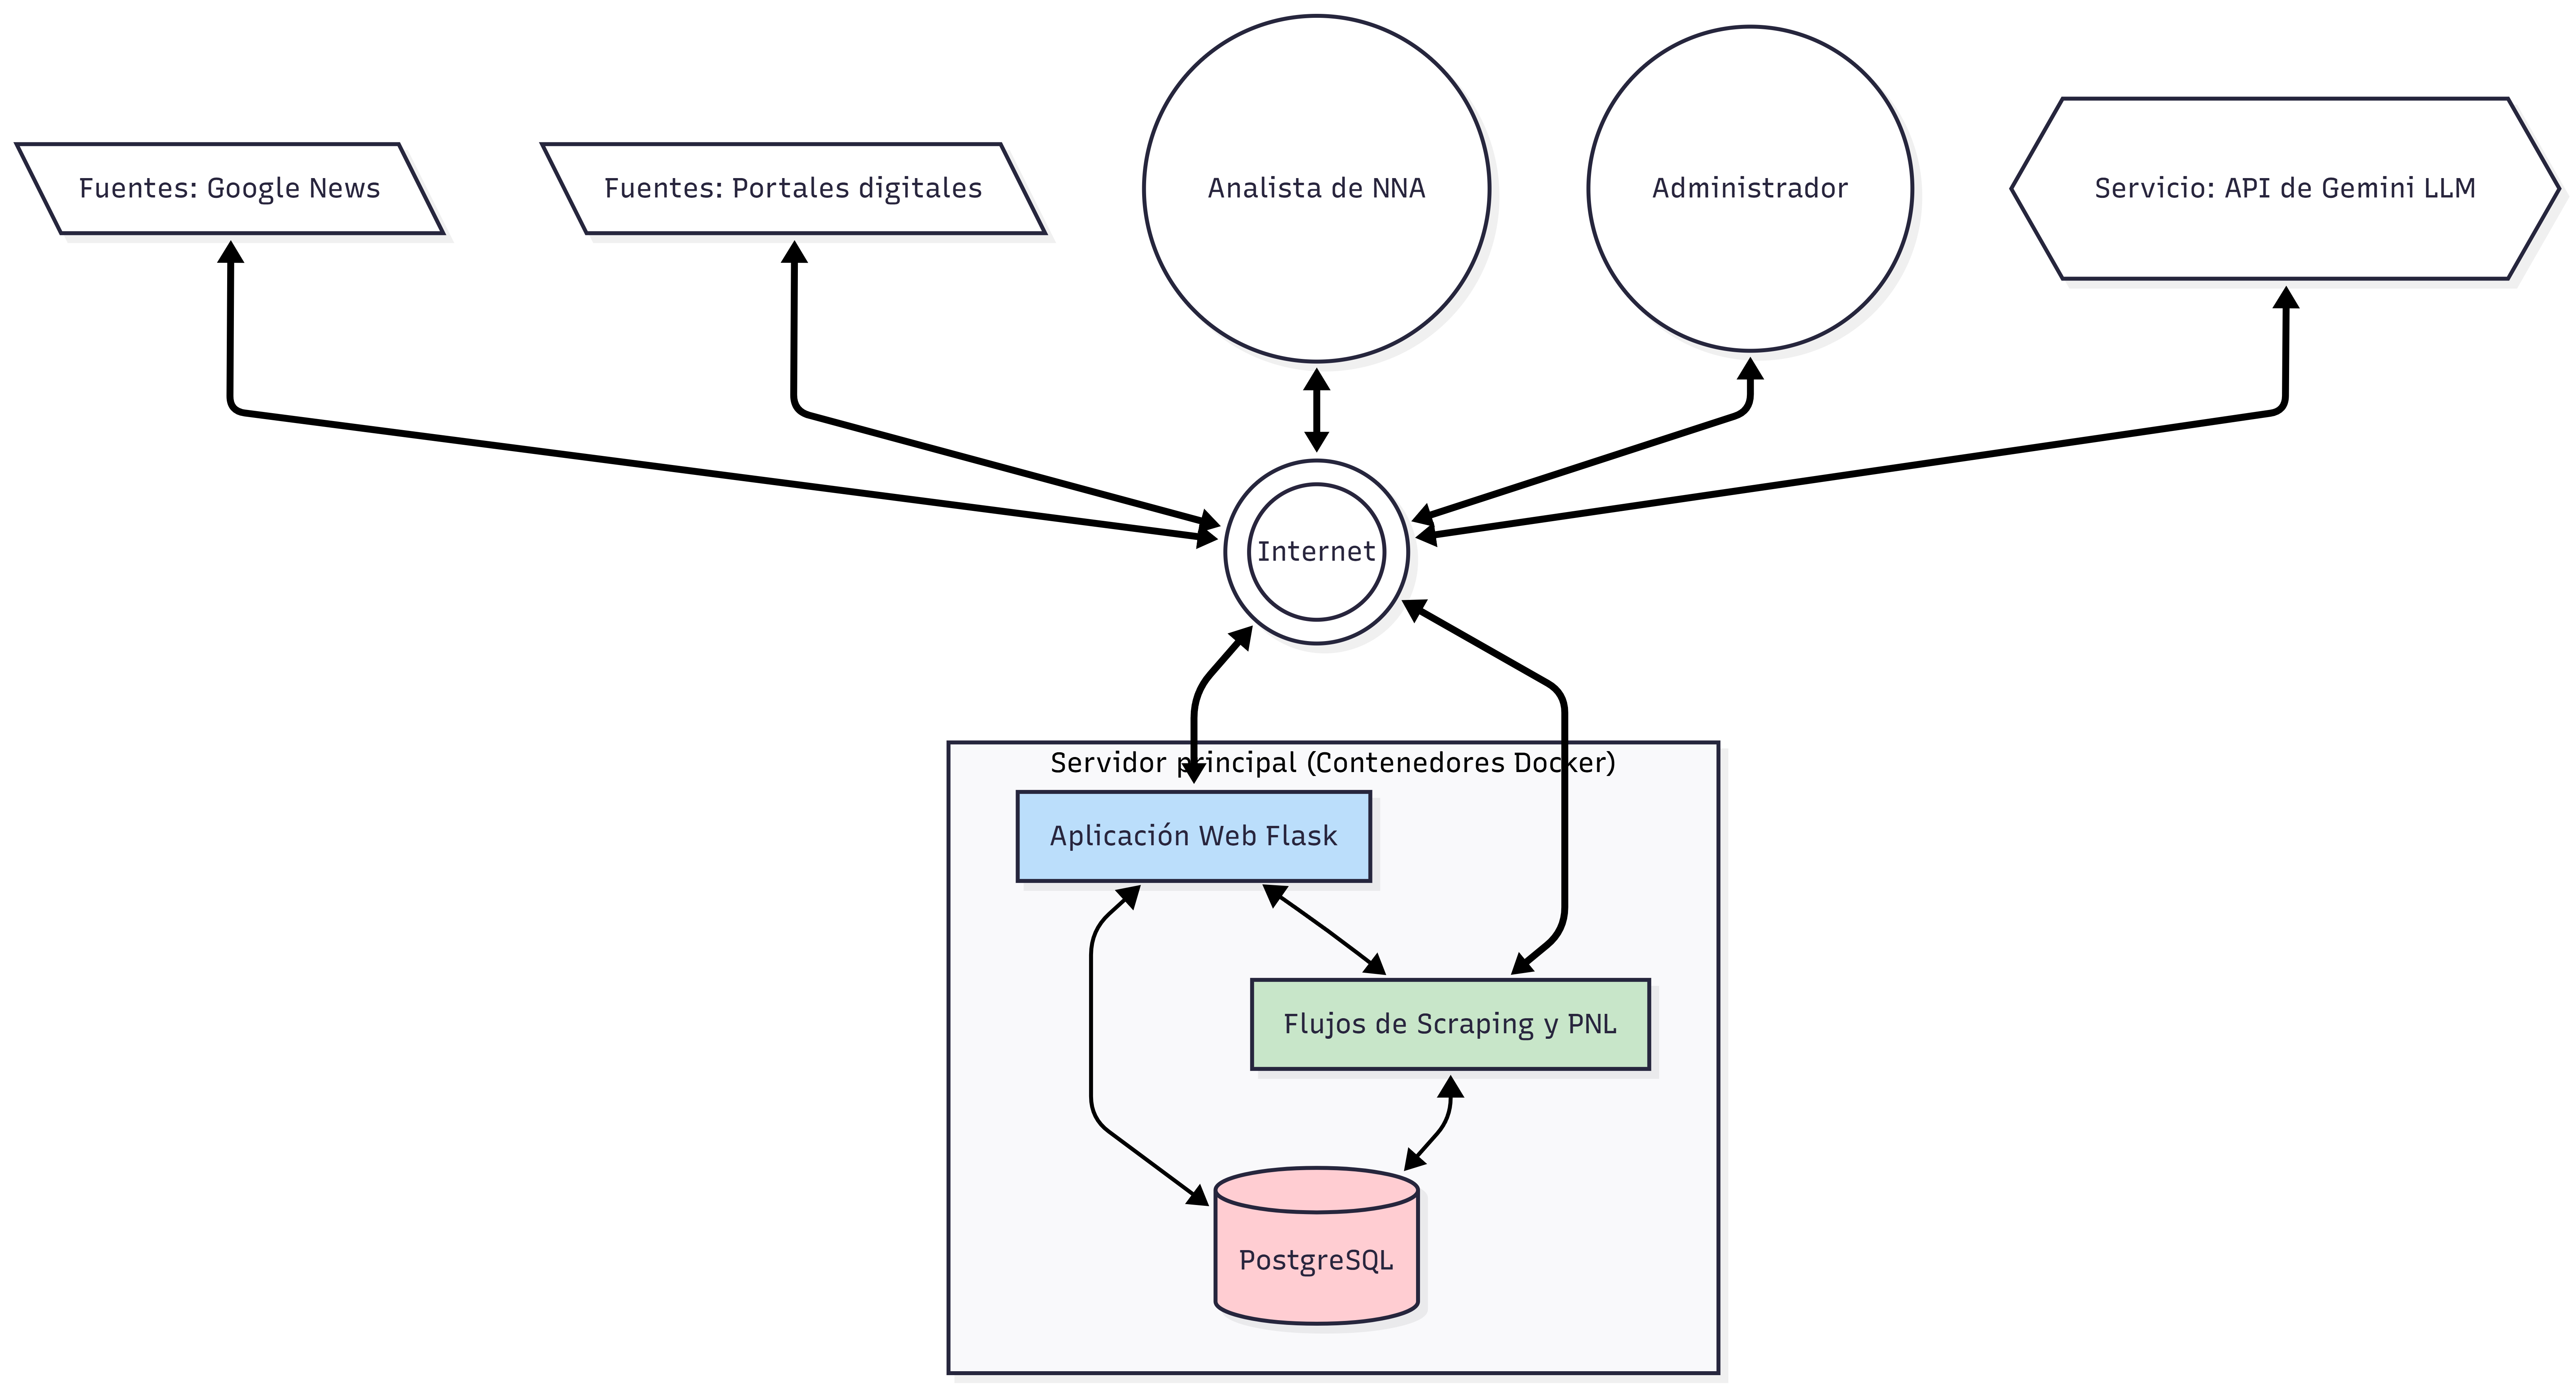
\includegraphics[width=\linewidth]{arquitecturascrap.png}
  \caption{Arquitectura de microservicios contenerizada. Tres contenedores
           Docker se comunican sobre la red privada \texttt{nna-network},
           garantizando aislamiento de recursos y persistencia de datos
           ante reinicios del sistema.}
  \label{fig:arquitectura}
\end{figure}

% ============================================================
\section{Resultados}

\subsection{Recolección y Deduplicación}

En el ciclo de validación final se procesaron $\approx$900~noticias brutas;
la cascada eliminó 213~duplicados: 89 por MD5 (10.5\%), 61 por Jaccard
(7.2\%), 43 por SimHash (5.1\%) y 20 por coseno TF-IDF (2.4\%), obteniendo
\textbf{634~noticias únicas}. Esto representa un incremento del 125\%
respecto a las 281~noticias del TT-1.

\subsection{Evaluación del Clasificador Escalonado}

Para validar el desempeño sobre datos no vistos durante el fine-tuning, se
construyó un conjunto de prueba ciego de 43~noticias por muestreo
segmentado. Dos anotadores independientes (un docente de la ESCOM y el
autor) etiquetaron cada noticia con protocolo binario. El acuerdo
inter-anotador fue $\kappa{=}0.91$ (\textit{casi perfecto} según Landis y
Koch~\cite{landis1977}); 2~noticias sin consenso fueron excluidas,
dejando $n{=}41$ para el cálculo de métricas~\cite{cohen1960}.

La \mbox{TABLA~\ref{tab:metricas}} resume los resultados. El clasificador
alcanzó un F1-Score de \textbf{0.85}, un Recall de \textbf{0.95} y una
tasa de falsos positivos del \textbf{30\%}, cumpliendo el umbral operativo
(${\leq}30\%$). La matriz de confusión arrojó VP~=~20, VN~=~14, FP~=~6,
FN~=~1; el único falso negativo corresponde a una noticia con redacción
ambigua sin mención explícita de víctimas menores.

\begin{table}[htbp]
\centering
\caption{Métricas del clasificador escalonado ($n{=}41$)}
\label{tab:metricas}
\renewcommand{\arraystretch}{1.25}
\begin{tabular}{lc}
\toprule
\textbf{Métrica} & \textbf{Valor} \\
\midrule
Precisión                          & 0.77 \\
Recall (Sensibilidad)              & 0.95 \\
F1-Score                           & 0.85 \\
Tasa de Falsos Positivos           & 30.0\% \\
$\kappa$ de Cohen (inter-anotador) & 0.91 \\
\bottomrule
\end{tabular}
\end{table}

\subsection{Distribución del Embudo Analítico}

El corpus de 634~noticias fue reducido secuencialmente: 409~superaron
la Capa~0 (64.5\%), 225 la Capa~1 (35.5\%), 128 la inferencia \BETO{}
con score~$>$~0.50 (20.2\%), de los cuales \textbf{27 fueron clasificados
como Alta relevancia} (4.4\%) y \textbf{101 como Media} (15.9\%). Los
27~casos de Alta correspondieron a eventos de orfandad verificables
manualmente.

\subsection{Agrupamiento y DeepInvestigator}

BERTopic generó 15~tópicos semánticos coherentes sobre las 634~noticias.
El \texttt{DeepInvestigator} completó el flujo de investigación sobre
15~noticias de Alta clasificación con tiempo promedio de 47\,s por caso
y generación correcta de fichas con contactos institucionales (DIF
municipal, Fiscalía competente). La TABLA~\ref{tab:topicos} presenta
los cinco tópicos de mayor frecuencia identificados por el modelo.

\begin{table}[htbp]
\centering
\caption{Top~5 tópicos identificados por BERTopic}
\label{tab:topicos}
\renewcommand{\arraystretch}{1.2}
\begin{tabular}{cp{3.2cm}c}
\toprule
\textbf{ID} & \textbf{Palabras clave (c-TF-IDF)} & \textbf{Frec.} \\
\midrule
0 & orfandad, hijos, madre, feminicidio, resguardo & 41 \\
1 & custodia, DIF, abuelos, tutela, menor           & 28 \\
2 & manifestación, colectivos, justicia, marcha     & 22 \\
3 & sentencia, juicio, agresor, carpeta, proceso    & 19 \\
4 & NNA, testigo, presencia, crimen, escena         & 14 \\
\bottomrule
\end{tabular}
\end{table}

\subsection{Evaluación Comparativa TT-1 / TT-2}

La \mbox{TABLA~\ref{tab:comparativa}} consolida el cumplimiento de los
objetivos cuantitativos definidos al inicio del TT-2.

\begin{table}[htbp]
\centering
\caption{Comparativa de métricas TT-1 vs.\ TT-2}
\label{tab:comparativa}
\renewcommand{\arraystretch}{1.2}
\begin{tabular}{p{2.0cm}p{1.1cm}p{1.6cm}p{1.6cm}}
\toprule
\textbf{Métrica} & \textbf{TT-1} & \textbf{Meta TT-2} & \textbf{P4 final} \\
\midrule
Falsos positivos & 60\%    & $\leq$30\%     & 30.0\% $\checkmark$ \\
Fuentes          & 10 RSS  & 45 RSS+GNews   & 45+GN+Stealth $\checkmark$ \\
Noticias únicas  & 281     & $>$500         & 634 $\checkmark$ \\
Motor PLN        & RegEx   & BETO ft.       & BETO Escalonado $\checkmark$ \\
Persistencia     & CSV     & PostgreSQL     & PostgreSQL ACID $\checkmark$ \\
\bottomrule
\end{tabular}
\end{table}

% ============================================================
\section{Conclusiones}

Se desarrolló e implementó un sistema de monitoreo inteligente que demuestra
la viabilidad de automatizar la identificación de \NNA{} en situación de
orfandad por feminicidio a partir de fuentes periodísticas digitales. Las
contribuciones técnicas principales son: (i)~la arquitectura de
clasificación neuro-simbólica escalonada que supera tanto los enfoques
puramente léxicos como los modelos Transformer en modo \textit{zero-shot},
y (ii)~la cascada de deduplicación multi-algoritmo que garantiza la
integridad del corpus. El F1-Score de 0.85 con Recall de 0.95 valida la
hipótesis de que la integración de reglas simbólicas de dominio sobre la
salida neuronal de \BETO{} es necesaria para dominios de alta especificidad.

\subsection{Trabajo Futuro}

Se identifican tres líneas prioritarias: (1)~\textbf{Active Learning}:
incorporar retroalimentación del analista para reentrenar el clasificador
de forma incremental; (2)~\textbf{Reentrenamiento en GPU}: el fine-tuning
actual se realizó en CPU con 8~GB RAM; hardware acelerado permitiría
explorar modelos de mayor capacidad (RoBERTa-es, mDeBERTa); y
(3)~\textbf{Extensión geográfica}: adaptar el catálogo de fuentes hacia
Centroamérica para ampliar el impacto del sistema.

% ============================================================
\section*{Reconocimientos}

Los autores agradecen a la Escuela Superior de Cómputo (ESCOM) del
Instituto Politécnico Nacional (IPN) por el apoyo institucional brindado
durante el desarrollo del Trabajo Terminal 2026-A135, así como a los
sinodales y profesores que enriquecieron el proyecto con su orientación
técnica y metodológica.

% ============================================================
\begin{thebibliography}{99}

\bibitem{sesnsp2023}
Secretariado Ejecutivo del Sistema Nacional de Seguridad Pública,
``Información sobre violencia contra las mujeres,''
Gobierno de México, Informe anual, 2023.
[En línea]. Disponible en: \url{https://www.gob.mx/sesnsp}

\bibitem{redim2022}
Red por los Derechos de la Infancia en México (REDIM),
``Infancia y feminicidio en México: impacto en niñas, niños y adolescentes,''
REDIM, Ciudad de México, Informe técnico, 2022.

\bibitem{onu2019}
Oficina del Alto Comisionado de las Naciones Unidas para los Derechos Humanos,
``Diagnóstico sobre la situación de los derechos humanos en México,''
ONU-DH México, 2019.

\bibitem{CaneteCFP2020}
J. Cañete, G. Chaperon, R. Fuentes, J.-H. Ho, H. Kang, y J. Pérez,
``Spanish Pre-trained BERT Model and Evaluation Data,''
en \textit{Proc. PML4DC at ICLR 2020}, Addis Abeba, Etiopía, 2020.

\bibitem{bertopic2022}
M. Grootendorst,
``BERTopic: Neural Topic Modeling with a Class-Based TF-IDF Procedure,''
\textit{arXiv preprint arXiv:2203.05794}, 2022.

\bibitem{guo2017calibration}
C. Guo, G. Pleiss, Y. Sun, y K. Q. Weinberger,
``On Calibration of Modern Neural Networks,''
en \textit{Proc. 34th Int. Conf. Machine Learning (ICML)},
Sydney, Australia, 2017, pp.~1321--1330.

\bibitem{cohen1960}
J. Cohen,
``A Coefficient of Agreement for Nominal Scales,''
\textit{Educational and Psychological Measurement},
vol.~20, no.~1, pp.~37--46, 1960.

\bibitem{landis1977}
J. R. Landis y G. G. Koch,
``The Measurement of Observer Agreement for Categorical Data,''
\textit{Biometrics}, vol.~33, no.~1, pp.~159--174, 1977.

\bibitem{anderson2019tls}
B. Anderson y D. McGrew,
``OS Fingerprinting: New Techniques and the Impact on Security Tools,''
en \textit{Proc. IEEE Security \& Privacy Workshops},
San Francisco, CA, EE.~UU., 2019, pp.~1--7.

\bibitem{bird2009nlp}
S. Bird, E. Klein, y E. Loper,
\textit{Natural Language Processing with Python}.
Sebastopol, CA: O'Reilly Media, 2009.

\bibitem{joachims1998text}
T. Joachims,
``Text Categorization with Support Vector Machines: Learning with Many
Relevant Features,''
en \textit{Proc. 10th European Conf. Machine Learning (ECML)},
Chemnitz, Alemania, 1998, pp.~137--142.

\bibitem{pressman2014}
R. S. Pressman y B. R. Maxim,
\textit{Software Engineering: A Practitioner's Approach}, 8th~ed.
Nueva York, NY: McGraw-Hill, 2014.

\end{thebibliography}

\end{document}
